%!TEX root = ../main.tex
%%%%%%%%%%%%%%%%%%%%%%%%%%%%%%%%%%
% Links:
%
% Difficulty:
% Companies: 
%%%%%%%%%%%%%%%%%%%%%%%%%%%%%%%%%%


%\begin{figure}
%	\centering
%	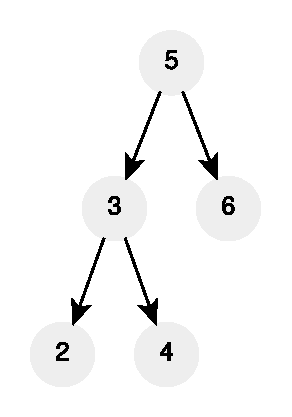
\includegraphics[width=\textwidth]{sources/longest_consecutive_sequence/images/example1}
%	\caption[Sample short cpation]{Sample Caption}.
%	\label{fig:longest_consecutive_sequence:example1}
%\end{figure}

\chapter{Longest consecutive sequence}
\label{ch:longest_consecutive_sequence}
\section*{Introduction}

\section{Problem statement}
\begin{exercise}
Write a function that, given a collection $L$ of integers returns the length of the longest sequence of consecutive numbers in $L$.
\label{example:longest_consecutive_sequence:exercice1}

	%example1
	\begin{example}
		\label{example:longest_consecutive_sequence:example1}
		\hfill \\
		Given $L=\{45,31,46,235,28,30,29,47\}$ the function return $4$; The longest sequence of consecutive number is $\{28,29,30,31\}$.		
	\end{example}

	%example2
	\begin{example}
		\label{example:longest_consecutive_sequence:example2}
		\hfill \\
		Given $L=\{8,2,7,5,0,1,4,6,3\}$ the function return $9$; $L$ contains all numbers from $0$ to $8$.				
	\end{example}

\end{exercise}

\section{Clarification Questions}

\begin{QandA}
	\item Does $L$ contains only positive numbers?
	\begin{answered}
		\textit{No, it might contain any number that fits a standard \inline{int}}.
	\end{answered}

	\item Can $L$ contain duplicates?
	\begin{answered}
		\textit{Yes, duplicates are allowed}.
	\end{answered}

	\item What is the maximum size of $L$?
	\begin{answered}
		\textit{$L$ might contain up to $10e6$ elements}.
	\end{answered}
	
\end{QandA}

%\section{Discussion}
%\label{longest_consecutive_sequence:sec:discussion}
\subsection{Solution using Sorting}
\label{longest_consecutive_sequence:sec:bruteforce}
Would this problem be easier if the input array was sorted to begin with? 
The answer to this question is yes, as, consecutive elements would appear one after the other and therefore, would be easy to check for sequences of consecutive elements with a single linear visit of the array.

For let's imagine for a second that the input of  Example \ref{example:longest_consecutive_sequence:example1} was sorted i.e. $L=\{28,29,30,31,45,46,47,235\}.$ It is easy to see that we have three sequences of elements with the first starting at the beginning of the array and ending after the first pair of elements at indices $x$ and $x+1$ s.t. $L[x+1]!= L[x]+1$, the second starting at index $x+1$ and ending at the next pair satisfying the conditions mentioned just above 9ending at element $47$). We can find the start and end indices of the third sequence similarly to the first two.
Therefore, one easy way to solve this problem would be to sort $L$ first and then to scan it and count the length of the consecutive sequences. 

Listing \ref{list:longest_consecutive_sequence:sorting} shows an implementation of this idea.


\lstinputlisting[language=c++, caption={$O(nlog(n))$ time and $O(1)$ space solution using sorting.},label=list:longest_consecutive_sequence:sorting]{sources/longest_consecutive_sequence/longest_consecutive_sequence_solution1.cpp}

The code works by first sorting and removing duplicates in $L$. Removing duplicates is not strictly necessary but it does makes the code after a little more simpler and clearer and does not make the overall time complexity worse. The variable \inline{curr_count} keeps track of the size of the current sequence of consecutive numbers. This number is incremented everytime the current element is exactly equal to the next minus one and reset to $1$ whenever this condition is not met. 
The maximum value registered by this counter will be the final answer that is returned.

The time complexity of this solution is $O(n log(n))$ as we sort the array and the subsequent while loop runs in linear time. 

The space complexity is $O(1)$.

\subsection{Linear time and space solution}
\label{longest_consecutive_sequence:sec:lineartime}
We can however avoind sorting and removing duplicates alltogether and solve this problem in linear time if we are willing to use also linear space.
The idea would be to build an undirected graph $G=(V,K)$ ($V$ being the nodes and $K$ the edges) from $L$ where we have one node for each element of $L$.
If we carefully connects these nodes in $V$ such that nodes corrensponding to consecutive elements are linked together than the result would be a graph with one or more connected components. Each connected component is a sequence of consecutive elements and therefore all we have to do is to visit each of these connected components and find ount the one with most nodes.

We know that we can visit a graph in linear time and therefore the only issue we have to make this solution work is being able to construct such a 
graph also in linear time. 
Lucklily also this step is easily achievable in linear time. We can represent $G$ with an hashmap mapping elements of $V$ to their respective successor and predecessor nodes in $V$ using a \inline{std::unordered_map<int, std::pair<std::optional<int>, std::optional<int>>>}; we use the first and second component of the pair to store the predecessor and successor elements, respectively. 
Also, we notice that \inline{std::optional<int>} is used to represent the fact that a node might not have a successor or a predecessor.

We can build $G$ bit by bit by scanning $L$ one element at the time and for each of its element $l$ we can check whether $l+1$ and $l-1$ are alredy present in $G$. 
When the predecessor $l-1$ of $l$ is present in $G$ all we have to do is to connect $l-1$ with $l$ in such a way that we can go from $l-1$ to $l$ by moving forward (via its successor link in its associated \inline{std::pair}) and that we can also go from $l$ to $l-1$ following $l$'s predecessor link.
Similarly, when $l+1$ is in $G$ we connect $l$ and $l+1$ but this time we make sure we can go from $l+1$ to $l$ via $l+1$'s predecessor link and from $l$ to $l+1$ via $l$'s successor link.
Eventually when we have visited $L$ entirely, all consecutive nodes are connected in one or more connected components. 

Figure \ref{fig:longest_consecutive_sequence:graph_example1} show how the graph would look like for the Example \ref{example:longest_consecutive_sequence:example1}. Figure \ref{fig:longest_consecutive_sequence:graph_example1_1} shows the same graph with grops belonging to the same connected components depicted one close to the other.
From these two figures it is clear to notice how we can visit and entire connected component and calculate its size  and that we can start the visit from each of its nodes.  

\begin{figure}
	\centering
	\begin{subfigure}[t]{0.99\textwidth}
		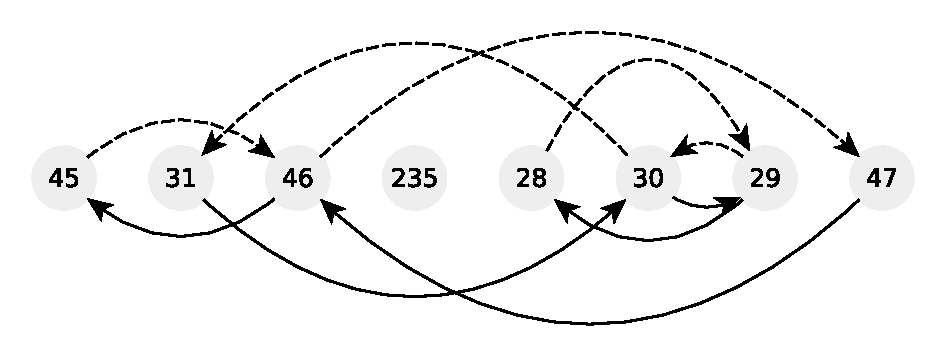
\includegraphics[width=1\linewidth]{sources/longest_consecutive_sequence/images/example_graph1}
		\caption{Graph representation of the Example \ref{example:longest_consecutive_sequence:example1}. Dotted edged represents successors links.}
		\label{fig:longest_consecutive_sequence:graph_example1}
	 \end{subfigure}
	\hfill
	\begin{subfigure}[t]{0.99\textwidth}
		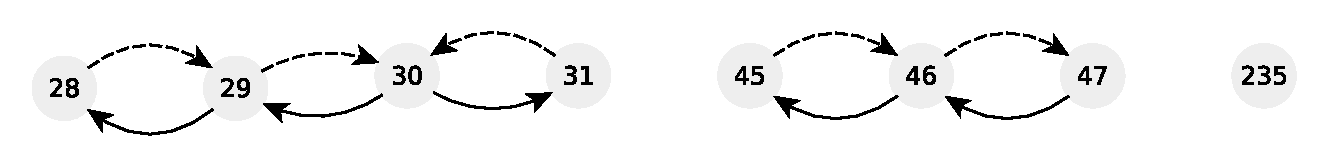
\includegraphics[width=1\linewidth]{sources/longest_consecutive_sequence/images/example_graph1_1}
		\caption{Graph shown in Figure \ref{fig:longest_consecutive_sequence:graph_example1} with nodes reordered to highlight the connected components.
		Dotted edged represents successors links.}
		\label{fig:longest_consecutive_sequence:graph_example1_1}
	 \end{subfigure}
	 \caption[]{}
	  \label{}
\end{figure}


An implementation of this strategy is shown in  Listing \ref{list:longest_consecutive_sequence:lineartime}.

\lstinputlisting[language=c++, caption={Linear time and linear space solution.},label=list:longest_consecutive_sequence:lineartime]{sources/longest_consecutive_sequence/longest_consecutive_sequence_solution2.cpp}

The code works in two distinct phases each implemented in its own function:
\begin{enumerate}
	\item \inline{build_graph}: where we construct the graph discussed above.
	\item \inline{find_longest_connected_component} where we take such a graph and we visit it.
\end{enumerate}

The graph building part is pretty straightforward and nothing more than connecting nodes that are consecutive is done here. 

The visit of the graph is possibly more interesting because we erase from the graph nodes  as we visit them so that a connected component is only visited once (otherwise what would happen in case the entire graph had only a single connected component? we would visit all of the graph for each and every element of $L$, causing the time complexity to skyrocket to quadratic time).

We try to start the visit of a connected component ech node $l$ of $L$ . If the the node we want to start the visit from has been already visited, it would not be present in $G$ and therefore we know it has been already considered. 
In case it yet to be visited then we visit the connected component starting from it counting how many steps we can make in the left and right direction. 
The lenght of the sequence would be the sum of the steps we can take to the left and to the right of $l$  plus $1$, to account for $l$ itself.

To count the step we can make in a given direction we use the function \inline{find_longest_connected_component} which simply follows the links in $G$ from a given starting node until we reach a dead end.

Listing \ref{list:longest_consecutive_sequence:lineartime} has linear time and space complexities.